\documentclass[12pt, a4paper, oneside]{ctexart}
\usepackage{amsmath, amsthm, amssymb, bm, color, framed, graphicx, hyperref, mathrsfs,float}
\usepackage{tcolorbox}
\usepackage{colortbl}
\usepackage{geometry}
\usepackage{booktabs}

\CTEXsetup[format={\Large\bfseries}]{section}
\title{\textbf{Review Notes: Data Mining}}
\author{Zeqiang Zhang}
\date{\today}
\linespread{1.5}
\definecolor{shadecolor}{RGB}{241, 241, 255}
\newcounter{problemname}
\newcounter{gnc}
\newenvironment{problem}{\begin{shaded}\stepcounter{problemname}\par\noindent\textbf{题目\arabic{problemname}. }}{\end{shaded}\par}

\newenvironment{zd}{\begin{shaded}\par\noindent\textbf{这一章的重点是:}}{\end{shaded}\par}
\newenvironment{solution}{\par\noindent\textbf{解答. }}{\par}
\newenvironment{note}{\par\noindent\textbf{题目\arabic{problemname}的注记. }}{\par}
\newenvironment{classnotes}{\begin{shaded}\par\noindent\textbf{相关讲义:}}{\end{shaded}\par}

\begin{document}

\maketitle

\newpage
\tableofcontents
\newpage
\section{统计学基础}
\subsection{Scaling of the data}
\begin{itemize}
    \item Nominal scale
    
    大小无意义
    \item Ordinal scale
    
    大小有意义,可以进行比较,但数据的差值无意义,因此不能进行加减。
    \item Interval scale
    
    数据的差值有意义,可以进行加减。但无绝对零点,因此不能进行乘除。
    \item Ratio scale
    
    有绝对零点,可以进行乘除。
\end{itemize}
\subsection{Evaluation of univariate data \& single features}
\begin{itemize}
    \item 频数(Absolute frequency)和频率(Relative frequency).
    \item 众数(mode):频数最大的特征。一个数据集可以有多个众数。
    \item 经验分布函数(empirical distribution function):$F(x)=\frac{\mbox{小于x的数据个数}}{\mbox{总数}}$
    
    经验分布函数是递增的阶跃函数。
    \item 分位数(Quantiles):
    \begin{itemize}
        \item 中位数(median):$x_{\frac{1}{2}}$
        \item 四分位数(quartile):$x_{\frac{1}{4}}$,$x_{\frac{1}{2}}$,$x_{\frac{3}{4}}$
    \end{itemize}
    \item Boxplot
    
    Median inside the box.

    1. and 3. quartil defining the box.

    注意outliers.
    \begin{figure}[htbp]
        \centering
        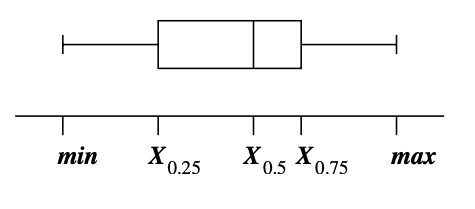
\includegraphics[width=0.5\textwidth]{boxplot.png}
        \caption{Boxplot}
    \end{figure}
    \item 计算数据的位置:
    \begin{itemize}
        \item 算数平均值(arithmetic mean):$\overline{x}=\frac{1}{n}\sum_{i=1}^{n}x_i$ 
        \item 加权平均值(weighted mean):$\overline{x}_w=\frac{1}{n}\sum_{i=1}^{n}x_i*w_i$ 
    \end{itemize}
    \item 计算数据的偏离程度:
    \begin{itemize}
        \item 方差(Variance):$s^2=\frac{1}{n-1}\sum_{i=1}^{n}{(x_i-\overline{x})}^2$
        \item 标准差(standard deviation):$s$
        \item 与中位数的平均偏差(Mean absolute deviation from median):
        
        $\frac{1}{n}\sum_{i=1}^{n}|x_i-\widetilde{x}_{0.5}|$
        \item 平均偏差(Mean difference):$\frac{1}{n^2}\sum_{i=1}^{n}\sum_{j=1}^{n}|x_i-x_j|$
        \item Quartil difference:$\widetilde{x}_{0.75}-\widetilde{x}_{0.25}$
        \item Range:$\max_i x_i - \min_i x_i$
        
        \begin{tcolorbox}
            记住英文名字和计算公式。注意Quartil difference不受极端值的影响,Range易受极端值影响。
        \end{tcolorbox}
    \end{itemize}
    \item 偏度(Skewness):
    \begin{itemize}
        \item Skewness: $g=\frac{1}{n}\sum_{i=1}^n{(\frac{x_i-\overline{x} }{s})}^3$
        \item Quartile skewness: $g_Q=\frac{(\widetilde{x}_{0.75}-\widetilde{x}_{0.5} )-(\widetilde{x}_{0.5}-\widetilde{x}_{0.25})}{\widetilde{x}_{0.75}-\widetilde{x}_{0.25}}$
    \end{itemize}
    \begin{tcolorbox}
        \begin{itemize}
            \item Skewness的公式不用记,Quartile skewness的公式最好记一下。
            \item $g>0$(or $g_Q>0$): right-skewed; $g<0$(or $g_Q<0$): left-skewed。
            \item 对称(Symmetric)一定$g=0$(or $g_Q=0$),但是$g=0$(or $g_Q=0$)不一定对称。
        \end{itemize}
    \end{tcolorbox}
    \begin{figure}[htbp]
        \centering
        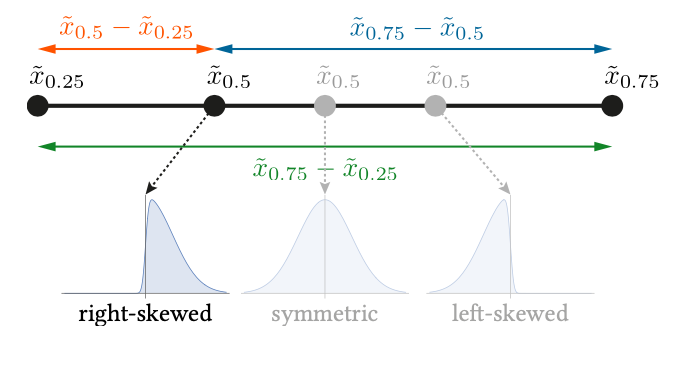
\includegraphics[width=0.8\textwidth]{skewness.png}
        \caption{偏度}
    \end{figure}
    \newpage
    \item (Assignment01) Measure和需要的scaling:
    
    \begin{table}[!htbp]
        \centering
        \label{Measure}
        \caption{Measure \& Required scaling}
    \begin{tabular}{cc}
        \toprule  
        Measure& Required scaling\\
        \midrule  
        Mode& Nominal \\
        Arithmetic mean $\overline{x} $&Interval  \\
        Quantile $\widetilde{x}_{0.25}$&Ordinal  \\
        Median $\widetilde{x}_{0.5}$&Ordinal \\
        Range $R$&Interval  \\
        Interquartile range $Q$&Interval  \\
        Variance $s^2$&Interval \\
        Skewness $g$&Interval  \\
        Quartile skewness $g_Q$&Interval \\
        \bottomrule 
    \end{tabular}
    
    \end{table}
\end{itemize}

\subsection{Evaluation of multivariate data}
\begin{itemize}
    \item 协方差(Covariance):$S_{XY}=\frac{1}{n-1}\sum_{i=1}^n(x_i-\overline{x} )(y_i-\overline{y} )$
    \begin{itemize}
        \item 协方差取值可以为任意实数。
        \item $S_{XY}>0$ 正相关;$S_{XY}<0$ 负相关。
    \end{itemize}
    \item 相关系数(Correlation coefficient):$r_{XY}=\frac{S_{XY}}{S_XS_Y}$
    \begin{itemize}
        \item 相关系数取值范围$[-1,1]$。
        \item $r_{XY}>0$ 正相关;$r_{XY}<0$ 负相关。$|r_{XY}|$越大,相关性越强。
        \item $X$和$Y$成一次函数关系时$|r_{XY}|=1$。
    \end{itemize}
    \item Contingency table: 表示变量的频率分布。
    
    假设$X$变量有$J$种取值,$Y$变量有$K$种取值,则Contingency table为一个$J \times K$的表格,其中$n_{jk}$表示$X$变量取第$j$个值,$Y$变量取第$k$个值的数据的个数(或频率)。
    
    通过该表格可以计算边缘分布(marginal frequencies),条件分布(conditional distribution)。
    \item 独立性(Independency): $X$和$Y$独立(descriptive independent),若$f_{jk}=f_j \cdot f_k$。
    \begin{tcolorbox}
        独立可以推导出$r_{XY}=0$,反之不成立。即独立一定不相关,不相关不一定独立。
    \end{tcolorbox}
    \item Rank order correlation coefficient 和 Correlation of nominal scaled data 
    
    应该不会考?没时间就不用看(slides: 69-72)。
\end{itemize}


\section{聚类分析}
\begin{itemize}
    \item Data matrix and distance matrix:
    \begin{itemize}
        \item Data matrix: data list
        \item Proximity (distance or similarity) matrix: where distances or
        similarities between pairs of units are given
    \end{itemize}
    \item Distance:
    \begin{itemize}
        \item Manhattan metric: $d_r(x,y)=\sum_{i=1}^n|x_i-y_i|$
        \item Euclidean metric: $d_r(x,y)=\sqrt{\sum_{i=1}^n{(x_i-y_i)}^2}$ (即几何距离)
        \item Hamming distance: Manhattan metric for Boolean space. (即对于两个布尔类型的数据,Hamming distance是两个数相应位数上的不同数字的个数)
    \end{itemize}
    \item Matching coefficients (slides 84)(这个要记住公式):
    \begin{itemize}
        \item Simple-matching-coefficient (SMC) = $\frac{n_{00}+n_{11}}{n}$(相同的数字的概率)
        \item Jaccard-coefficient (JC) =$\frac{n_{11}}{n-n_{00}}$(全1的数字占有1的数字之比)
        \item Rao-Russel-coefficient (RRC)=$\frac{n_{11}}{n}$(全1的数字的概率)
    \end{itemize}
    \item 处理缺失的数据(slides 87)
\end{itemize}
\subsection{Hierarchical Clustering}
\subsubsection{Agglomerative clustering(自底向上)}
\begin{itemize}
    \item 算法:给定一个数据集
    \begin{enumerate}
        \item 计算距离矩阵(data matrix)
        \item 找到有最小距离的两个聚类,将它们合并成一个新的聚类
        \item 计算新的聚类与其他聚类的距离,更新距离矩阵
        \item 重复执行,直到所有的数据合并成一个聚类
    \end{enumerate}
    \item 因此,重点问题在于如何定义两个聚类之间的距离:
    \begin{itemize}
        \item Single linkage clustering (SCL)
        
        新聚类与其他聚类的距离为原两个聚类与其他聚类的距离的较小者,即:$$d_c(C_F,C_r)=\min\{d_c(C_{i^*}, C_r), d_c(C_{j^*}, C_r)\}$$
        \begin{tcolorbox}
            Chaining-effect: 对于SCL,如果两个距离较远类别的数据中间有数据连接,这两个类别的数据很可能被划分为同一类。(示意图和解释:slides 102)
        \end{tcolorbox}
        \item Complete-Linkage-Clustering (CLC)
        新聚类与其他聚类的距离为原两个聚类与其他聚类的距离的较大者,即:$$d_c(C_F,C_r)=\max\{d_c(C_{i^*}, C_r), d_c(C_{j^*}, C_r)\}$$
        \begin{tcolorbox}
            SCL和CLC的对比:判断两类是否会合并时,SCL关注两类间的最小距离,CLC关注两类间的最大距离。(slides 104:判断哪种情况是SLC,哪种情况是CLC,及原因。或给定树状图,判断哪个来自SCL,哪个来自CLC。)
        \end{tcolorbox}
        \item Group average algorithm:
        
        新聚类与其他聚类的距离为两个聚类里所有元素距离的加权平均:$$d_c(C_F,C_r)=\frac{m_{i^*}}{m_{i^*}+m_{j^*}}d_c(C_{i^*}, C_r)+\frac{m_{j^*}}{m_{i^*}+m_{j^*}} d_c(C_{j^*}, C_r)$$
        \item Unweighted average algorithm

        Group average algorithm的近似。$$d_c(C_F,C_r)=\frac{1}{2}d_c(C_{i^*}, C_r)+\frac{1}{2} d_c(C_{j^*}, C_r)$$
        \item Centroid algorithm:
        
        计算两个聚类的距离,先计算两个聚类的中心(所有点的平均值),然后再计算两个中心的距离。新聚类的中心是两个原聚类的加权平均。

        \item Median algorithm:
        
        Centroid algorithm的近似。新聚类的中心是两个原聚类的算数平均(即假设两个原聚类有相同数目的点)。



    \end{itemize}
\end{itemize}
\subsubsection{Divisive clustering(自顶向下)}
\subsection{Partitional Clustering}
\begin{itemize}
    \item Variance criterion: 
    
    寻找一种聚类方式,使得方差之和最小(因此每一个聚类内部数据的差异最小)。(slides 113)
    \item k-means clustering
    
    \begin{enumerate}
        \item 首先随机选取聚类的中心点
        \item 将数据分配到最近的聚类中心点
        \item 对于每一个聚类,根据分配的数据重新计算中心点
        \item 重复执行上述算法,直到不再改变
    \end{enumerate}
    \item ANOVA:
    
    \begin{itemize}
        \item $T=W+B$,T是total scatter matrix, W 是 within scatter matrix, B 是 between scatter matrix。
        \item 取矩阵的迹,得$tr(T)=tr(W)+tr(B)$。可以理解为$tr(T)$是数据总体的方差,$tr(W)$是每一个聚类内部的方差,$tr(B)$是聚类与聚类之间的方差。
        \item 数据总体的方差$tr(T)$是定值,因此,减小每一个聚类内部的方差$tr(W)$就是要增大聚类与聚类之间的方差$tr(B)$。(即每一类里的数据尽可能相似,类与类之间的数据尽可能不同。)
    \end{itemize}

    \item Exchange Clustering Algorithm
    
    \begin{enumerate}
        \item 初始化聚类。
        \item 选一个点,改变这个点所属的聚类。如果改变之后与改变之前相比,方差之和减小了,就接受改变,否则拒绝改变。
        \item 重复执行第二步直到算法结束。
        \item 如果重复足够多次,每个点都会属于距离自己最近的聚类中心。
    \end{enumerate}
\end{itemize}
\subsection{Fuzzy cluster analysis}
\begin{itemize}
    \item Crisp clustering 和 Fuzzy clustering:
    \begin{itemize}
        \item Crisp clustering: 每一个数据都确定的分给某一个聚类中心
        \item Fuzzy clustering:每一个数据在一定程度上属于每一个聚类中心,可以理解为概率。
    \end{itemize}
    例如如果有三个聚类中心$C_1,C_2,C_3$,数据$x$属于$C_1$即为Crisp clustering,数据$x$对于三个聚类点的归属程度分别为$[0.8,0.1,0.1]$即为Fuzzy clustering。Crisp clustering可视为Fuzzy clustering的一种特殊情况(即归属程度为$[1,0,0]$)。

    \item Constraints for fuzzy membership: (概率约束)
    \begin{enumerate}
        \item $f_{\mu,j} \in [0,1]$
        \item $\sum_j f_{\mu,j}=1$
    \end{enumerate}

    \item (Slides 137)已知数据和fuzzy matrix,如何计算聚类中心:思路类似于加权平均数。
    \item (Slides 138-140)已知数据和聚类中心,对于每一个数据,如何计算fuzzy membership:这是一个约束条件的最优化问题,Slides中用拉格郎日乘数法计算。应该不用记公式,也不用看懂推导过程。
    \item 通过上两步,我们得到了更新聚类中心和更新fuzzy membership的方法。因此我们可以执行Fuzzy-k-means算法:
    \begin{itemize}
        \item 首先随机选取聚类的中心点。
        \item 根据聚类中心,分配数据(计算fuzzy membership)。
        \item 根据fuzzy matrix, 更新聚类中心。
        \item 重复执行上述算法。
    \end{itemize}
\end{itemize}
\subsection{Neuronal clustering}
\begin{itemize}
    \item Competitive learning:
    
    \begin{enumerate}
        \item 初始化聚类。
        \item 选择一个点,计算这个点离得最近的聚类中心($j$)。
        \item 更新离这个点最近的聚类中心($j$)。
        \item 重复执行上述算法。
    \end{enumerate}

    \item Kohonen algorithm:
    
    大致流程与Competitive learning相同,不同地方在于选择一个点,并且计算这个点离得最近的聚类中心($j$)之后,下一步不仅仅更新($j$),而是更新所有的聚类中心。每一个聚类中心的更新幅度与该聚类中心和聚类中心$j$的距离有关。例如:
    \begin{itemize}
        \item Neural Gas:
        
        \begin{enumerate}
            \item 选择一个点,计算这个点与所有聚类中心的距离,并且进行排序。
            \item 根据排序,更新所有的聚类中心。
        \end{enumerate}
    \end{itemize}

    \item LVQ1 Algorithm: 带有标签的监督学习
    \begin{enumerate}
        \item 初始化聚类。
        \item 选择一个点,计算这个点离得最近的聚类中心($j$)。
        \item 更新离这个点最近的聚类中心($j$):如果分类是正确的,就+;分类错误,就-。
        \item 重复执行上述算法。
    \end{enumerate}  
\end{itemize}
\begin{zd}
    \begin{enumerate}
        \item Agglomerative clustering中SCL和CLC的计算、绘制树状图、判断树状图属于哪种算法。SCL和CLC的区别,SCL的chaining effect。
        \item Partitional clustering中理解Variance criterion。k-means clustering的计算过程。
        \item Fuzzy cluster: 理解fuzzy cluster,fuzzy cluster和crisp clustering的区别,fuzzy membership的约束条件。
    \end{enumerate}
\end{zd}
\section{数据可视化与降维}
\subsection{Principal component analysis (PCA)}
PCA的想法是找到一个方向,使得该方向上数据的方差最大(因此该方向上数据分得更开,即保留了原始数据集的更多信息)。
\begin{enumerate}
    \item 给定一个数据集$X(n\times d)$。假定数据集每个维度上的均值都是0,否则用数据集减去均值得到新的数据集。
    \item 对于一个$d$维基向量$v$($v$的模长为1,即$\left\|v\right\|_2=1$),将$x_i$向$v$投影,有$\alpha_i=v^Tx_i$。
    \item 因为$X$在每一个维度上的均值为0,因此有$\overline{\alpha}=0 $。我们的目的是寻找一个方向$v$,使得$\alpha$的方差最大。
    \item $\alpha$的方差计算公式为:$$\begin{aligned}
        \sigma_v^2&=\sum_{i=1}^n{(\alpha_i-\overline{\alpha})}^2=\sum_{i=1}^n\alpha_i^2=\sum_{i=1}^n{(v^Tx_i)}^2\\
        &=\sum_{i=1}^nv^Tx_ix_i^Tv=v^T(\sum_{i=1}^nx_ix_i^T)v=v^T\mathbf{C}v\\
    \end{aligned}$$
    \item 因此现在的问题是寻找$v$,使得$v^T\mathbf{C}v$最小,约束条件是$v^Tv=1$。我们可以使用拉格郎日乘数法。
    \item (slides: 181)计算发现$v$是$\mathbf{C}$的特征向量,而$\sigma_v^2$是对应的特征值。
\end{enumerate}
因此,PCA算法为:
\begin{enumerate}
    \item 将数据集减去数据集的均值,使得数据集每个维度均值为0。
    \item 计算$\mathbf{C}=X^TX$,
    \item 计算$\mathbf{C}$的特征向量和特征值,并按照特征值从大到小排序。
    \item 将数据集投影到前$d^\prime$个特征向量。
\end{enumerate}
\subsection{Multi dimensional scaling}
MDS的想法是,对于一个数据集$X$,计算数据集的距离矩阵$D^X$。将$X$映射到可视化空间$Y$后,计算新空间中的距离矩阵$D^Y$。寻找一种映射方式使得$D^X$尽可能接近$D^Y$(因此这种方法会保留数据点之间的距离信息)。

$D^X$与$D^Y$的差异用stress function来描述,定义为:$$S=\sum_{i=1}^n\sum_{j=1}^n{(\Phi [d^X(x_i,x_j)]-\Phi[d^Y(y_i,y_j)])}^2$$,其中$\Phi$是单调递增函数。

因此,可以用incremental update rule来更新$\mathbf{y}$,即:$$y_i^\prime=y_i-l\cdot \frac{\partial S}{\partial y_i}$$其中$l$是learning rate。

如果Y是二维空间,距离使用欧拉距离,即$d^Y(y_i,y_j)=d^2(y_i,y_j)={(y_i-y_j)}^2$,那么:$$\begin{aligned}\frac{\partial S}{\partial y_i}&=2\sum_{i=1}^n{(\Phi [d^X(x_i,x_j)]-\Phi[d^2(y_i,y_j)])}\cdot(-\Phi^\prime[d^2(y_i,y_j)])\cdot(-2(y_i-y_j))\\&=-4\sum_{i=1}^n\Phi^\prime[d^2(y_i,y_j)]{(\Phi [d^X(x_i,x_j)]-\Phi[d^2(y_i,y_j)])}\cdot(y_i-y_j)\end{aligned}$$(4放在了$l$,即186页的公式的推导。应该不用记,理解这里的计算方法是incremental update rule。)
\subsection{$t$-Distributed Stochastic Neighbor Embedding}
$t$-SNE的目的是保留相对位置信息(即相邻关系)。计算方法与MDS基本相同,不同的是在$t$-SNE,我们计算的不是距离矩阵,而是相对位置关系。定义$$p_{j|i}=\frac{e^{-{\frac{\left\|\mathbf{x}_i-\mathbf{x}_j\right\|_2}{2\sigma_i^2}}}}{\sum_{k\neq i}e^{-{\frac{\left\|\mathbf{x}_i-\mathbf{x}_k\right\|_2}{2\sigma_i^2}}}}\text{,} p_{ij}=\frac{p_{i|j}+p_{j|i}}{2}$$ 
\begin{itemize}
    \item $p_{j|i}$可以理解为$j$是$i$的邻居点的概率。
    \item $\sigma_i$控制的是$i$数据点考虑的范围,与Perplexity有关。Perplexity可以理解为考虑的周围数据点的个数。因此Perplexity是一个确定的数,而对于每一个数据点,根据Perplexity我们可以确定相应的$\sigma_i$。
\end{itemize}
$P$和$Q$的距离用KL散度来计算,即:$$D_Q(P)=\sum_i\sum_j\log_2(\frac{p_{ij}}{q_{ij}})$$
\begin{zd}
    \begin{itemize}
        \item PCA、MDS和$t$-SNE三种算法及区别(2018考试题)。
        \begin{enumerate}
            \item 目的不同。PCA目的是寻找方差最大的方向,MDS试图在投影空间保持距离信息,$t$-SNE试图在投影空间保持相邻信息。
            \item PCA是确定的算法,MDS和$t$-SNE有随机性(每次运行结果可能不同)。
            \item 计算方法不同。PCA通过计算矩阵特征值和特征向量,MDS和$t$-SNE通过incremental update rule。
        \end{enumerate}
    \end{itemize}
\end{zd}
\section{关联规则}
\begin{itemize}
    \item Support 和 Confidence:
    
    \begin{itemize}
        \item Support: item或关联规则的频率
        \begin{itemize}
            \item $Support(Y)=\frac{\text{物品}Y\text{出现的次数}}{n}$
            \item $Support(Y\rightarrow Z)=Support(Y\cup Z)=\frac{\text{物品}Y\text{和}Z\text{同时出现的次数}}{n}$
        \end{itemize}
        \item Confidence:关联规则成立的概率
        \begin{itemize}
            \item $Confidence(Y\rightarrow Z)=\frac{Support(Y\cup Z)}{Support(Y)}$
        \end{itemize}
    \end{itemize}
\end{itemize}
\subsection{A priori Algorithm}
\begin{enumerate}
    \item 寻找item sets $X$,使得$support(X)\geqslant s_{min}$。
    \begin{enumerate}
        \item $H_1=\{Y\text{: the item sets with 1 elements}\}$
        \item $I_n=\{Y \in H_n: support(Y)\geqslant s_{min}\}$
        \item 若$I_n$为空集,结束;若$I_n$不为空集,$H_{n+1}=\{Y\cup Y^\prime: Y \in I_n \text{ and } Y^\prime \notin \text{ with }|Y^\prime|=1\}$
        \item 重复执行上述算法。
    \end{enumerate}
    \item 确定关联规则$X\rightarrow Y$,使得$confidence(X\rightarrow Y)\geqslant k_{min}$。
    \begin{itemize}
        \item 先从$|Y|=1$开始,如果满足条件就逐步增加$|Y|$。
    \end{itemize}
\end{enumerate}

\section{分类}
\subsection{Decision tree}
决策树的思路是每次根据单个的特征进行分组,下一步继续考虑其它特征再次分组,直到每一组标签都可以被确定。描述一种分类好或者不好的指标是Impurity measures,每次分组所使用的指标为可以带来最大Impurity gain的指标。
\begin{itemize}
    \item Impurity measures:
    \begin{itemize}
        \item Breiman’s conditions:
        \begin{enumerate}
            \item 若对所有的$j$,$p_j=\frac{1}{L}$,$Q(P)$取得最大值。
            \item 若集合中只有一类数据,$Q(P)$取得最小值。
            \item 对称性:交换数据标签的顺序,$Q(P)$不变。
        \end{enumerate}
        \item 常用的impurity measures:
        \begin{itemize}
            \item misclassification index: $Q_m(p)=1-\max_jp_j$
            \item Gini index: $Q_g(p)=1-\sum_{i=1}^Lp_i^2$
            \item entropy index: $Q_e(p)=-\sum_{i=1}^Lp_i\log_2p_i$
        \end{itemize}
    \end{itemize}
    \item Impurity gain:
    
    当使用一个特征将一个集合$R$分成$B$个子集合$R_1,R_2,\cdots R_B$后,Impurity gain定义为:
    $$\Delta Q = Q(R)-\sum_{i=1}^Bp_{R_i}Q(R_i)$$其中,$p_{R_i}$是$R_i$的频率。
    \item Pruning(剪枝):
    \begin{itemize}
        \item 为什么要剪枝:
        
        为了避免过拟合(overfitting)。数据集中的错误数据可能导致模型对新数据分类准确性下降。

        \item 怎样剪枝:
        
        限制决策树节点的个数或者深度。
    \end{itemize}
\end{itemize}
\subsection{Prototype based classifiers}
\begin{itemize}
    \item $k$-nearest-neighbour($k$-NN):
    
    对于一个给定的新数据点,计算该数据点与训练集中所有数据点的距离,找到最近的$k$个数据点(通常$k$为奇数)。这$k$个数据点中标签的众数就是新数据点的标签。
    \begin{itemize}
        \item $k$-NN算法无须训练。
        \item $k$-NN算法计算过程花费较高(因为每次都要算新数据点和所有数据点的距离)。
    \end{itemize}
\end{itemize}
\subsection{Linear classification}
线性分类器:$z=f(w^Tx+w_0)$。$w$和$w_0$是参数,$f$是一个二值函数。例如$w^Tx+w_0>0,z=1;w^Tx+w_0<0,z=-1$。把$w_0$扩展到$w$里面,并且把$x$扩展一维$1$,可以写成$z=f(w^Tx)$
\begin{itemize}
    \item Perceptron:
    \begin{enumerate}
        \item 初始化$w$。
        \item 对于每一个数据,判断分类器是否正确分类:$\delta = (y-f(w^Tx))$。
        \item 如果分类错误,就更新分类器参数:$w:=w+\delta x$。
    \end{enumerate}
    (slides 241-242在证明只要数据集可分,这个算法可以在有限次数内收敛。不用管他。)
    \item Support Vector Learning:
    
    SVM算法是Perceptron算法的特例。在Perceptron算法中,我们找到了一条直线将数据集分开,在SVM算法中,我们不仅希望找到这么一条直线,还希望这条直线距离我们的数据点最远。
    \begin{figure}[htbp]
        \centering
        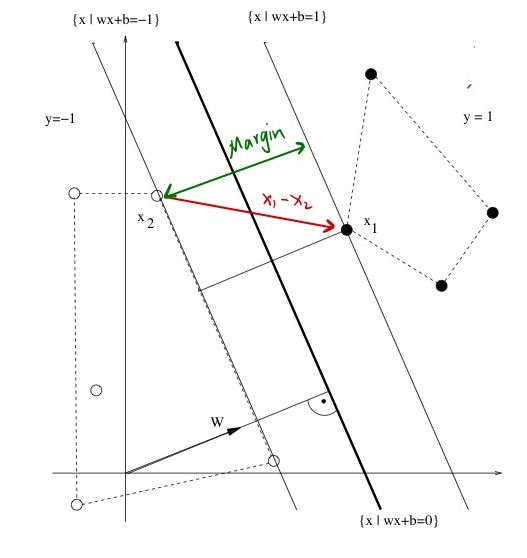
\includegraphics[width=0.9\textwidth]{dm-244.jpg}
        \caption{SVM}
    \end{figure}
    如图所示,分类器的表达式为$w^Tx+w_0$,其中$w^T$表示分界线的斜率,$w_0$表示分界线的位置。我们总能找到一个$w_0$,使得分界线处于正中间的位置。因此我们现在希望确定分界线的斜率,使得中间的间隔尽可能的大。

    假设我们现在已经有了一个$w$,如图所示,$x_1$和$x_2$是离分界线最近的点,我们有$w^Tx_1+w_0=\delta$,$w^Tx_2+w_0=-\delta$。我们将$w$替换为$\frac{w}{\delta}$,$w_0$替换为$\frac{w_0}{\delta}$,就有了$w^Tx_1+w_0=1$,$w^Tx_2+w_0=-1$。

    两式相减,得$w^T(x_1-x_2)=2$。对于直线方程$w^Tx_2+w_0=0$,它的法向量的方向为$w$,因此法向量为$\frac{w}{\left\|w\right\|}$。所以间隔为$x_1-x_2$在直线方程法向量方向的投影,即$\frac{w^T}{\left\|w\right\|}(x_1-x_2)=\frac{2}{\left\|w\right\|}$。因此我们的目标是最大化$\frac{2}{\left\|w\right\|}$。
    
    即:最小化$$\varphi (w)=\frac{{\left\|w\right\|}^2}{2}$$约束条件是对于任意的$\mu$,有$$y^\mu(w^Tx^\mu+w_0)\geqslant 1$$

    同样地,这是一个有约束的最优化问题,可以用拉格郎日乘数法计算。计算结果在(slides 247)。支持向量(support vectors)是位于间隔边界上的点,它们将对分类器产生影响。$w$是支持向量的线性组合。(slides 248-249是$w$和$w_0$的计算过程,不用看。)SVM的特点在于:
    \begin{itemize}
        \item 分类的间隔更大。
        \item 只需要考虑支持向量。
    \end{itemize}

    不可分问题:应该不会考。(引入新的优化量,目的是让间隔尽可能地大,同时不可分的点尽可能靠近间隔边缘。)
\end{itemize} 
% \left\|w\right\|
\subsection{Evaluation}
\begin{itemize}
    \item 为了验证算法的有效性,需要将数据集划分为训练集和测试集。在训练集上训练算法,在测试集上验证算法。但是对于规模较小的数据集,不适合这么做。
    \item Cross-Validation method:将数据集平均分成$k$份,计算$k$个分类器,每一次其中一份作为测试集,其余作为训练集,最后综合$k$次的结果来评估算法。
\end{itemize}
\begin{zd}
    \begin{itemize}
        \item 决策树比较重要:如何计算impurity measures,impurity gain;绘制决策树。
        \item $k$-NN算法比较简单。
        \item 线性分类器Perceptron比较好算,可以出计算题。SVM不会出计算题,理解SVM的目的和Support Vector的作用就可以。
        \item 验证,测试集和训练集,理解Cross-Validation method方法。(回归的验证方式类似)
    \end{itemize}
\end{zd}
\section{回归}
有一个未知的映射$X\rightarrow Y$。回归算法的目的是寻找一个函数,来模拟这个映射。即寻找$f(x)$,使得误差$\left\|f(x)-y\right\|$最小。
\subsection{Linear regression}
\begin{itemize}
    \item 一维线性回归(最小二乘法):
    
    拟合误差为:$$E=\sum_{i=1}^n{(ax_i+b-y_i)}^2$$
    $E$对$a$和$b$求偏导,可得:$$a=\frac{s_{xy}}{s^2_x}\text{ , }b=\overline{y}-a \overline{x}$$
    拟合直线经过点$(\overline{x}, \overline{y})$。

    \item 多维问题:
    
    拟合误差为:$E=\left\|Y-Xw\right\|$
    \begin{itemize}
        \item 如果$X$是可逆的,$w=X^{-1}Y$,此时$E=0$。
        \item 如果$X$不可逆,求$X$的伪逆矩阵,即$X^+={(X^TX)}^{-1}X^T$。$w=X^{+}Y$。
        \item 如果$X^TX$是奇异矩阵:slides 263.
    \end{itemize}

    \item 带有基函数的线性回归:
    
    $f(x)$是基函数的线性组合,即$f(x)=\sum_kw_kh_k(x)$。相当于从$X$根据基函数计算新的数据集$H$,拟合参数$w=H^+Y$。
    
\end{itemize}
\subsection{Nonlinear regression}
$f(x)=\sum_kw_kh_{c_k}(x)$。与带有基函数的线性回归区别在于函数$h(x)$中带有未知参数$c$。可用梯度下降算法求解。
\subsection{Regression based classification}
可以用回归方法解决分类问题。(例如有$L$个类别,我们拟合$L$个函数$f_1(x),f_2(x),\cdots,f_L(x)$,其中$f_i(x)$的值域是$[0,1]$。$f_i(x)$可以视为$x$与类别$i$的关系强度。)
\begin{zd}
    线性回归及带有基函数的线性回归。
    \begin{itemize}
        \item 一维情况下的计算。
        \item 判断什么是带有基函数的线性回归,什么是非线性回归。(如果基函数是确定的,就是带有基函数的线性回归,如果函数里有参数,就是非线性回归。)
        \item 带有基函数的线性回归的$H$矩阵。
    \end{itemize}
\end{zd}


\end{document}